\documentclass{beamer}

%%%%%%%%%%%%%%%%%%%%%%%%%%%%%%
\title{Steps C: surrogate models}
\author[M. Baudin]{Michaël Baudin\\Chu Mai}

% Copyright (C) 2012 - 2013 - EDF R&D - Michael Baudin

\setbeameroption{hide notes}
%\setbeameroption{show notes}
%\setbeameroption{show only notes}
%\mode<presentation>{\usetheme{EDF09}}

\usetheme{EDF09}
\useoutertheme{infolines}

\usepackage[T1]{fontenc}
\usepackage[utf8]{inputenc}
\usepackage{lmodern}

\usepackage[french]{babel}
\uselanguage{French}
\languagepath{French}

% Scilab macros
\newcommand{\sciobj}[1]{\texttt{#1}}
\newcommand{\scifile}[1]{\texttt{#1}}

% Python macros
\newcommand{\pyobj}[1]{\textcolor{blue}{\texttt{#1}}}

\def\RR{\mathbb{R}}
\def\NN{\mathbb{N}}
\def\bx{{\bf x}}

% To highlight source code
\usepackage{listings}
\definecolor{darkgreen}{rgb}{0,0.5,0}
\definecolor{violet}{rgb}{0.5,0,1}
\lstset{
  % general command to set parameter(s)
   basicstyle=\scriptsize\ttfamily, %
   keywordstyle=\color{violet}\bfseries,%
   commentstyle=\color{darkgreen}\bfseries,%
   showspaces=false,%
   stringstyle=\color{red}\bfseries
}

\hypersetup{
    %bookmarks=true,         % show bookmarks bar?
    %unicode=false,          % non-Latin characters in Acrobat�s bookmarks
    %pdftoolbar=true,        % show Acrobat�s toolbar?
    %pdfmenubar=true,        % show Acrobat�s menu?
    %pdffitwindow=false,     % window fit to page when opened
    %pdfstartview={FitH},    % fits the width of the page to the window
    %pdftitle={My title},    % title
    %pdfauthor={Author},     % author
    %pdfsubject={Subject},   % subject of the document
    %pdfcreator={Creator},   % creator of the document
    %pdfproducer={Producer}, % producer of the document
    %pdfkeywords={keyword1} {key2} {key3}, % list of keywords
    %pdfnewwindow=true,      % links in new window
    colorlinks=true,       % false: boxed links; true: colored links
    %linkcolor=red,          % color of internal links (change box color with linkbordercolor)
    %citecolor=green,        % color of links to bibliography
    %filecolor=magenta,      % color of file links
    urlcolor=blue           % color of external links
}

\graphicspath{{./Figures/}}



\begin{document}

%%%%%%%%%%%%%%%%%%%%%%%%%%%%%%%%%%%%%%%%%%%%%%%%%%%%%%%%%%%%%%%%%%%%%%%%%%%%%

\begin{frame}
\titlepage
  
\begin{center}

\includegraphics[height=0.2\textheight]{edf.jpg}
\hspace{1cm}

\includegraphics[height=0.2\textheight]{Maison_Simulation_LOGO.jpg}
\hspace{1cm}

\includegraphics[height=0.2\textheight]{PRACE_LOGO.jpg}
\end{center}

\end{frame}

%%%%%%%%%%%%%%%%%%%%%%%%%%%%%%%%%%%%

\begin{frame}
\frametitle{Introduction}

\begin{itemize}
\item The goal of this course is to introduce the main surrogate methods used in 
steps C. 

\item Principles of surrogate models, cross-validation, coefficient of predictability, over-fitting.

\item Linear regression, polynomial chaos, kriging.

\item The emphasis is not on maths. 

\item Instead, we feed the intuition with graphics. 
\end{itemize}

\end{frame}

%%%%%%%%%%%%%%%%%%%%%%%%%%%%%%%%%%%%

\begin{frame}
\begin{multicols}{2}
  {\tableofcontents[hideallsubsections]}
\end{multicols}
\end{frame}

%%%%%%%%%%%%%%%%%%%%%%%%%%%%%%%%%%%%

\section{Metamodels}

\subsection{Definition, construction and validation}

\begin{frame}[t]{Metamodel - Definition}

\begin{center}
 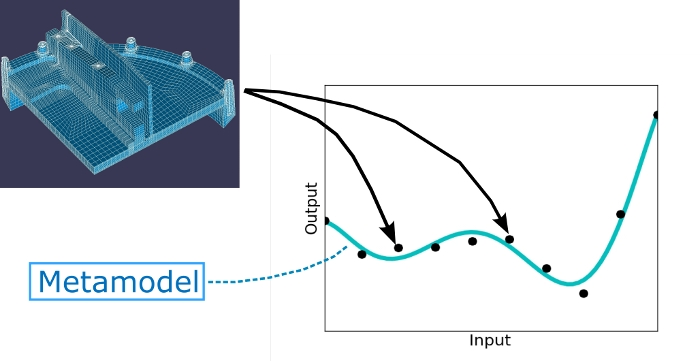
\includegraphics[height=3.2cm]{resp_surf_sketch.jpg}
\end{center}

A metamodel is an approximation model that mimics the behavior of a computationally expensive simulator by training on \emph{observations (data)} of the latter.

\end{frame}
%%%%%%%%%%%%%%%%%%%%%%%%%%%%%%%%%%%%

\begin{frame}[t]{Metamodel - Definition}

Model:
\begin{itemize}
\item Expensive simulator: 
$$
\boldsymbol{Y} \; = \; \boldsymbol{g}(\boldsymbol{X})
$$
\item $\boldsymbol{X} \in\RR^{n_X}$ : input vector
\item $\boldsymbol{Y}\in\RR^{n_Y}$ : output vector
\end{itemize}
   
Metamodel: 
$$ 
\widetilde{\boldsymbol{Y} } \; 
= \; \tilde{\boldsymbol{g}}(\boldsymbol{X}, \boldsymbol{\theta}), 
$$
where $\boldsymbol{\theta}$ is the vector of parameters

By definition, two requirements of a metamodel $\tilde{\boldsymbol{g}}$ are:
\begin{itemize}
\item Accurate when predicting away from known observations
\item Cheaper to evaluate than the primary simulator
\end{itemize}

\end{frame}

%%%%%%%%%%%%%%%%%%%%%%%%%%%%%%%%%%%%

\begin{frame}[t]{Metamodel - Objectives}

\begin{itemize}
\item Show functional relationships between input parameters and the output quantity of interest: impacts of variables 
% \item Augment results from single, expensive simulations: results can be predicted without use of the primary simulator; a continuous predictive function instead of discrete observations
\item Optimize the output quantity of interest: determine configurations that maximize the response or achieve specifications or customer requirements
\item Replace the primary simulator in uncertainty propagation 
(surrogate model):  e.g. in sensitivity analysis
%\item Multi-fidelity, multi-level approach: metamodel used as a bridge between a simple but inaccurate code and a more accurate but slower counterpart.
\end{itemize}

\end{frame}

\begin{frame}[t]{Major steps for constructing a metamodel}
 
\begin{center}
 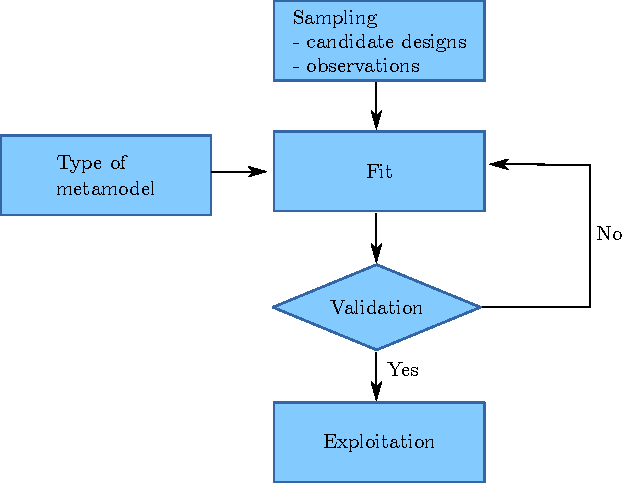
\includegraphics[width=0.7\textwidth]{metamodel_scheme.pdf} 
\end{center}

\end{frame}

%%%%%%%%%%%%%%%%%%%%%%%%%%%%%%%%%%%%

\begin{frame}[t]{Major steps for constructing a metamodel}

{\bf Sampling (define an experimental design):} 
\begin{itemize}
\item A number of possible candidate designs are generated
\item The designs are launched with the primary simulator
\end{itemize}

{\bf Constructing the metamodel:}
\begin{itemize}
\item A type of metamodel is selected (among several available options)
\item The metamodel is fitted to the available data
\item The metamodel is validated (yes or no)
	\begin{itemize}
	\item if yes: stop,
	\item otherwise, reject the model.
	\end{itemize}
\end{itemize}

\end{frame}

%%%%%%%%%%%%%%%%%%%%%%%%%%%%%%%%%%%%

\begin{frame}[t]{Major steps for constructing a metamodel}

If the model is rejected:
\begin{itemize}
 \item change method for fitting: e.g. use advanced regression technique instead of least squares errors,
 \item change metamodel parameters: e.g. increase polynomial degree,
 \item increase the sample size if the model is not accurate enough or interesting behavior is not observed,
 \item change the type of metamodel: e.g. polynomial chaos instead of second-order polynomial response surface
\end{itemize}	     

\end{frame}

%%%%%%%%%%%%%%%%%%%%%%%%%%%%%%%%%%%%

\section{Some types of metamodels}
\begin{frame}[t]{Some types of metamodels}

There are different metamodels available:
\begin{itemize}
\item Polynomial models 
\item Polynomial chaos models 
\item Kriging
\item Neural networks, 
\item etc...
\end{itemize}

They all require to:
\begin{itemize}
\item tune the parameters $\btheta$: \emph{training}, 
\item assess the quality of the prediction: \emph{validation}.
\end{itemize}

\end{frame}

%%%%%%%%%%%%%%%%%%%%%%%%%%%%%%%%%%%%

\section{Training and validation}
\begin{frame}[t]{Training and validation}

Creating a metamodel involves two steps.
\begin{enumerate}
\item Train: estimate the coefficients which fits to the data,
\item Test: quantify the predictability.
\end{enumerate}

\emph{But}, we must avoid overfitting: we must be able 
to predict datasets that have not been used to train the metamodel 
(more on this topic later).

One solution is to use cross-validation.
\begin{itemize}
\item Split the sample into a train sub-sample and a test sub-sample,
\item Train the metamodel on the train sample,
\item Test the metamodel on the test sample.
\end{itemize}

\begin{center}
 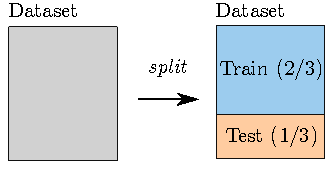
\includegraphics{train_test_cross_validation.pdf}
\end{center}

\end{frame}

%%%%%%%%%%%%%%%%%%%%%%%%%%%%%%%%%%%%

\begin{frame}[t]{Training and validation}

Assume that the output $y\in\RR$ is a scalar, i.e. $n_Y = 1$. 

Let $\left\{\bx^{(j)}_t\right\}_{j=1,...,n}$ an i.i.d. sample 
of the random vector $\bX$ that we use for training the 
metamodel. 

We denote by $g$ the model and $\tilde{g}$ the metamodel. 

For $j=1,...,n$, let 
$$
y^{(j)}_t = g\left(\bx^{(j)}_t\right), \qquad 
\tilde{y}^{(j)}_t = \tilde{g}\left(\bx^{(j)}_t\right)
$$
 be the outputs of the model and metamodel 
on the training set.
\end{frame}

%%%%%%%%%%%%%%%%%%%%%%%%%%%%%%%%%%%%

\begin{frame}[t]{Training and validation}

The Root Mean Squared Error is: 
$$
RMSE
= \left( \frac{1}{n} \sum_{j=1}^n \left( y^{(j)}_t - \tilde{y}^{(j)}_t \right)^2 \right)^{1/2}.
$$

A low RMSE is better. 
The $R^2$ coefficient is: 
$$
R^2(g(\bx_t),\tilde{g}(\bx_t)) 
= 1 - \frac{ \sum_{j=1}^n \left( y^{(j)}_t - \tilde{y}^{(j)}_t \right)^2}
{ \sum_{j=1}^n \left( y^{(j)}_t - \bar{y}_t \right)^2 }
$$
where $\bar{y}_t = \frac{1}{n} \sum_{i=1}^n y^{(j)}_t$. 
We usually have $R^2$ from 0 to 1, but a value $<0$ or $>1$ can occur. 
A value lower than zero indicates a poor prediction: $R^2 \approx 1$ 
is better. 

The coefficient quantifies the part of the variance which is predicted by the 
model. It is the improvement of the metamodel with respect to the 
mean prediction. 

\end{frame}

%%%%%%%%%%%%%%%%%%%%%%%%%%%%%%%%%%%%

\begin{frame}[t]{Training and validation}

Denote $\left\{\bx^{(j)}_v\right\}_{j=1,...,n}$ the 
validation sample. 

The goal of this sample is to test the metamodel on a dataset 
that was not used for training.

Let $g(\bx_v)$ and $\tilde{g}(\bx_v)$ the outputs of the 
model and metamodel on the validation sample.

The $Q^2$ predictability coefficient is defined as the $R^2$ 
applied to the validation sample:

$$
Q^2 = R^2(g(\bx_v),\tilde{g}(\bx_v)).
$$

A suggestion of decision rule:
\begin{itemize}
\item $Q^2>0.95$: accept the metamodel,
\item otherwise: try to improve the metamodel or reject it.
\end{itemize}

\end{frame}

%%%%%%%%%%%%%%%%%%%%%%%%%%%%%%%%%%%%

\begin{frame}[t]{Graphical validation}

\begin{center}
 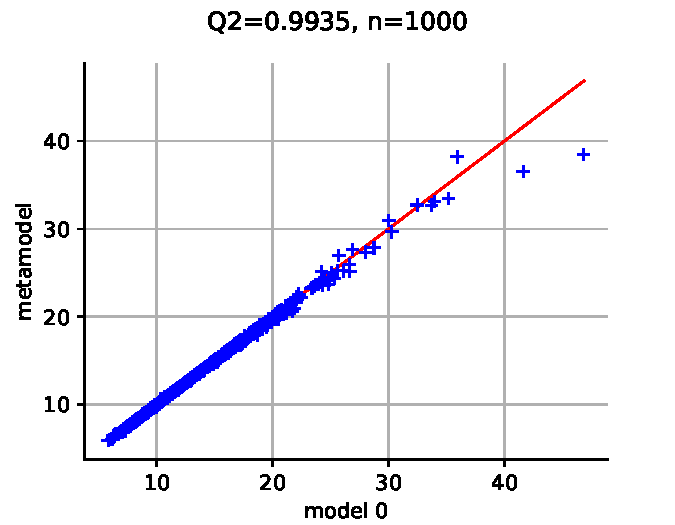
\includegraphics[width=0.7\textwidth]{surrogate-predictivity.pdf}
\end{center}

\end{frame}

%%%%%%%%%%%%%%%%%%%%%%%%%%%%%%%%%%%%
\section{Overfitting}

\begin{frame}[t]{Overfitting}

Overfitting is the fact that the surrogate model fits to the 
training sample, but predicts poorly on new points. 

\begin{itemize}
\item Any surrogate has coefficients tuned on the training sample.
\item More coefficients generally reduce the error on the training sample 
\item \emph{but} may increase the error on the validation sample.
\end{itemize}

There is a bias-variance trade-off to solve:
\begin{itemize}
\item More coefficients may reduce the variance (seen on the training sample), 
\item but may increase the bias (revealed on the validation sample).
\end{itemize}

\end{frame}
%
%%%%%%%%%%%%%%%%%%%%%%%%%%%%%%%%%%%

\begin{frame}[t]{Overfitting: example}

\begin{example}
We least linear least squares with a polynomial (\cite{bishop1995neural}, 
p.11). 
\begin{itemize}
\item We have 10 points on the [0,1] interval, produced by 
adding a small noise to the sine function. 
\item We approximate it with linear regression based on polynomial 
canonical basis.
\end{itemize}
\end{example}

\begin{center}
 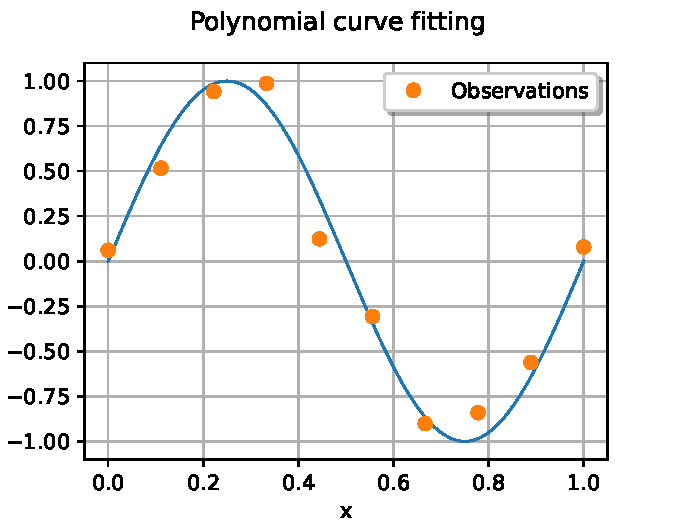
\includegraphics[width=0.40\textwidth]{overfitting-function-sample.pdf}
\end{center}

\end{frame}

%%%%%%%%%%%%%%%%%%%%%%%%%%%%%%%%%%%

\begin{frame}[t]{Overfitting: example}

We use linear least squares to fit a degree 4 polynomial (5 coefficients).

\begin{center}
 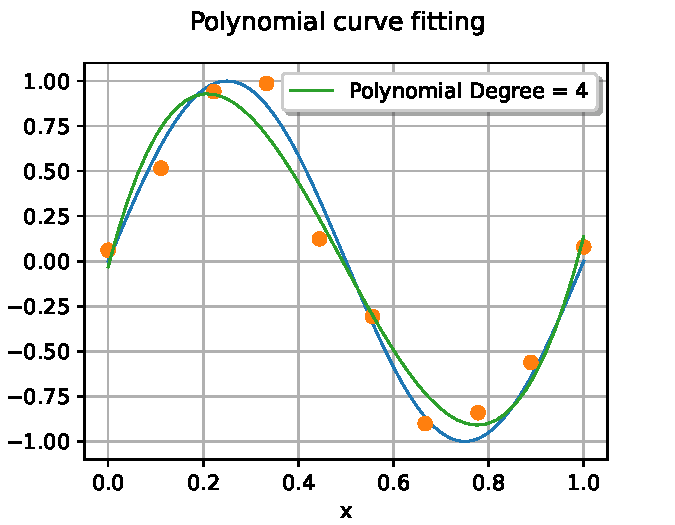
\includegraphics[width=0.7\textwidth]{overfitting-polynomial-degree-4.pdf}
\end{center}

\end{frame}

%%%%%%%%%%%%%%%%%%%%%%%%%%%%%%%%%%%

\begin{frame}[t]{Overfitting: example}

Increasing the degree does not always reduce the generalization error. 

\begin{center}
 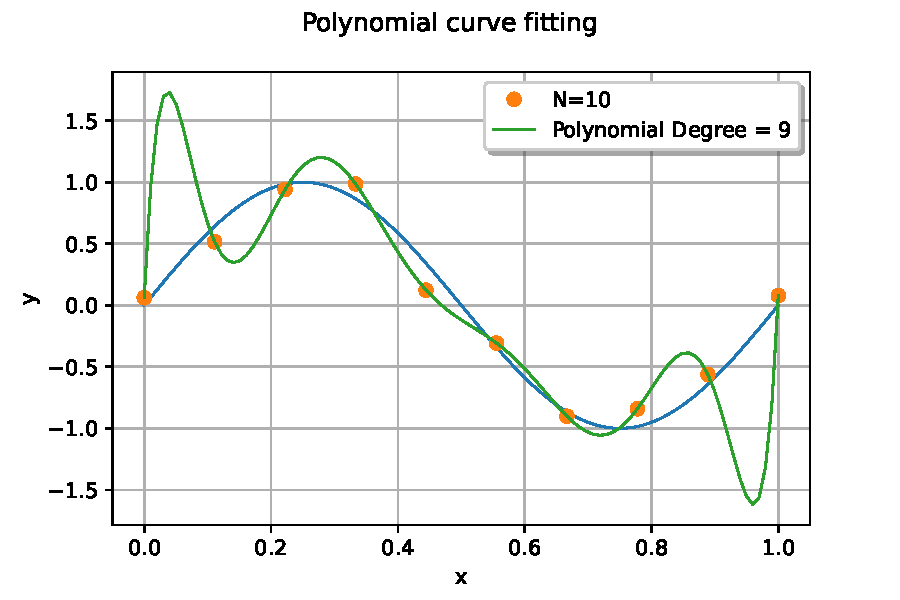
\includegraphics[width=0.75\textwidth]{overfitting-polynomial-degree-9.pdf}
\end{center}

\end{frame}

%%%%%%%%%%%%%%%%%%%%%%%%%%%%%%%%%%%

\begin{frame}[t]{Overfitting: example}

When we increase the degree, the root mean square error (RMSE) 
first decreases, then increases. 

\begin{center}
 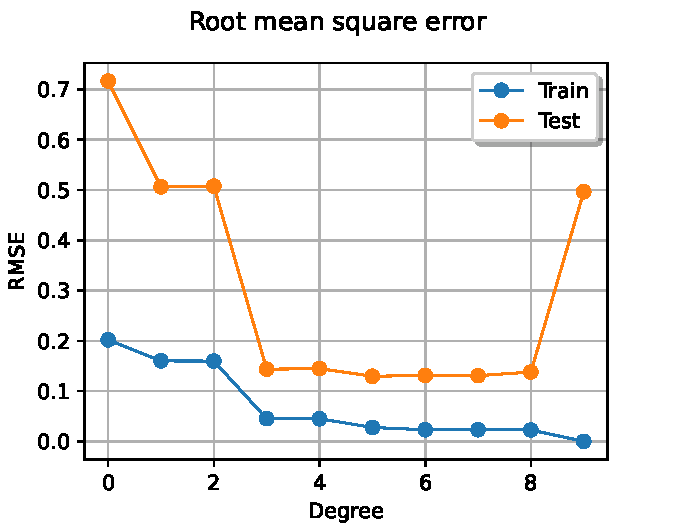
\includegraphics[width=0.6\textwidth]{overfitting-RMSE.pdf}
\end{center}

\end{frame}

%%%%%%%%%%%%%%%%%%%%%%%%%%%%%%%%%%%

\begin{frame}[t]{Overfitting: example}

Adding points to the training sample reduces the validation error, ...

\begin{center}
 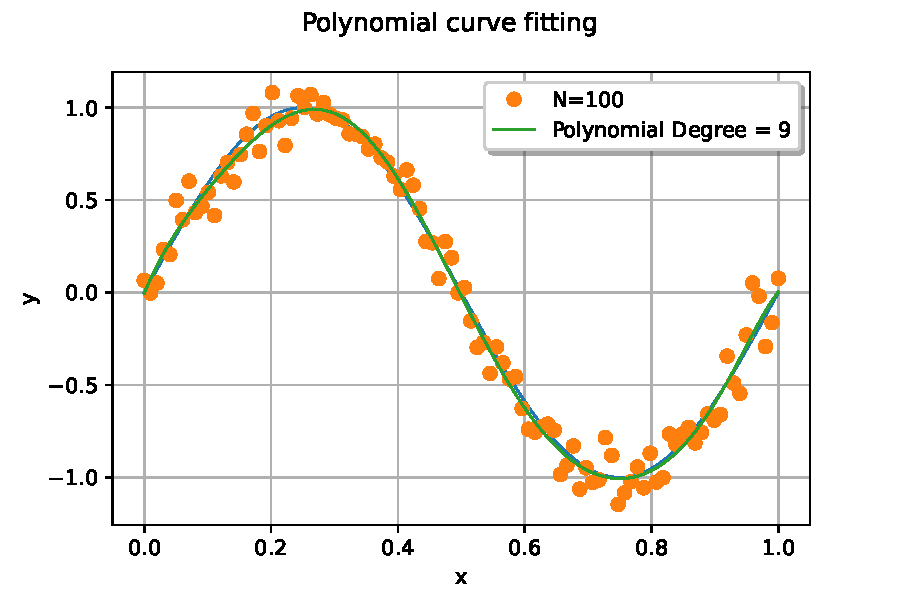
\includegraphics[width=0.7\textwidth]{overfitting-increase-sample-degree-9.pdf}
\end{center}

... but this is not always possible, e.g. the computer code may require 
costly simulations. 

\end{frame}

%%%%%%%%%%%%%%%%%%%%%%%%%%%%%%%%%%%

\begin{frame}[t]{Polynomial chaos example}

\begin{example}
\begin{itemize}
\item Consider the cantilever beam example $Y  = \dfrac{F\, L^3}{3 \, E \, I}$
with independent marginals: E: Beta, F: Lognormal, L: Uniform, 
I: Beta.

\item We approximate it with \emph{sparse} polynomial chaos: the model 
selection limits the number of coefficients in the model.
\end{itemize}

\end{example}

\begin{center}
 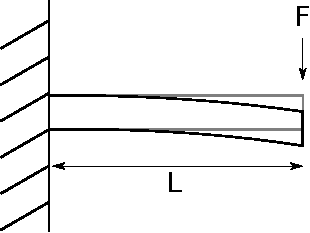
\includegraphics[width=0.35\textwidth]{poutre.pdf}
\end{center}

\end{frame}

%%%%%%%%%%%%%%%%%%%%%%%%%%%%%%%%%%%

\begin{frame}[t]{Polynomial chaos example}

Questions:
\begin{itemize}
\item How to set the sample size $n$ ?
\item How to set the polynomial degree $d$ ?
\end{itemize}

Method \cite{Gratiet2016}:
\begin{itemize}
\item Generate a training sample sample with size $n$ (e.g. $n=10$)
\item Generate a validation sample with size 1000.
\item Compute the $Q^2$. 
\item Repeat this experiment 50 times: get 50 $Q^2$ coefficients 
representing the variability of the $Q^2$ coefficient depending on the 
sample. 
\item We plot this sample of $Q^2$ coefficients in a boxplot: median, 
first quartile (25\%) and third quartile (75\%). 
\end{itemize}
\end{frame}

%%%%%%%%%%%%%%%%%%%%%%%%%%%%%%%%%%%

\begin{frame}[t]{Polynomial chaos example}

Left: n=10, Right: n=20.

\begin{center}
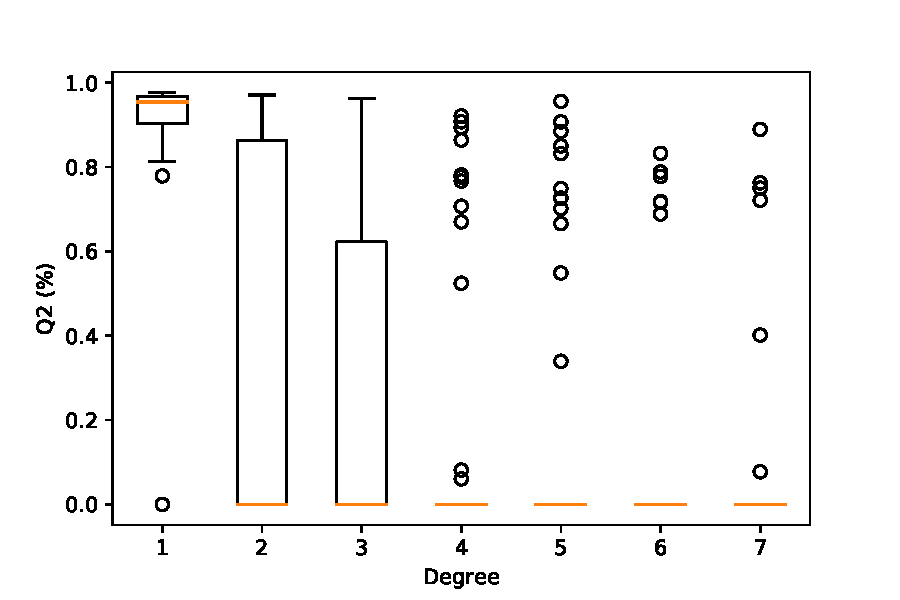
\includegraphics[width=0.45\textwidth]{chaos-poutre-N10-various-degrees.pdf}
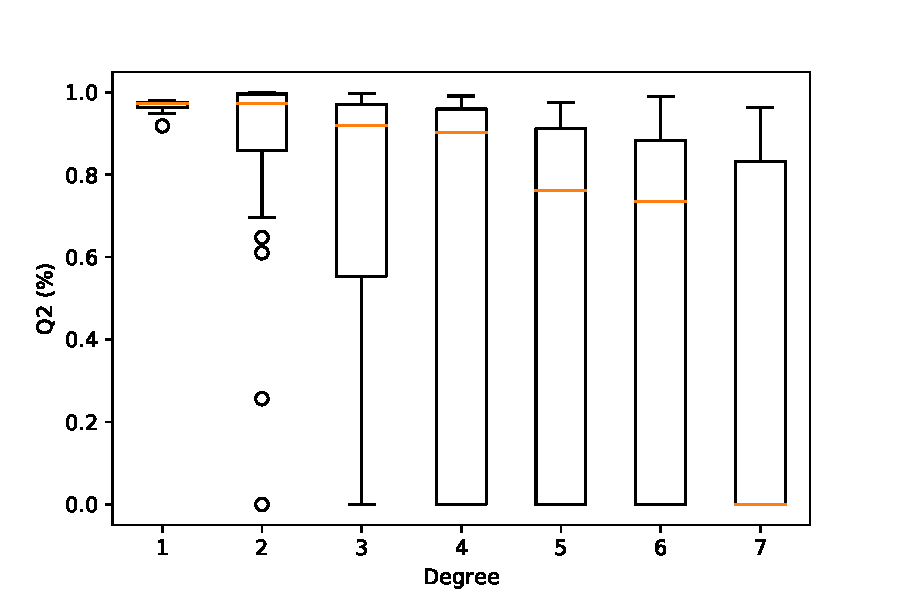
\includegraphics[width=0.45\textwidth]{chaos-poutre-N20-various-degrees.pdf}
\end{center}

\end{frame}

%%%%%%%%%%%%%%%%%%%%%%%%%%%%%%%%%%%

\begin{frame}[t]{Polynomial chaos example}

Left: n=30, Right: n=40.

\begin{center}
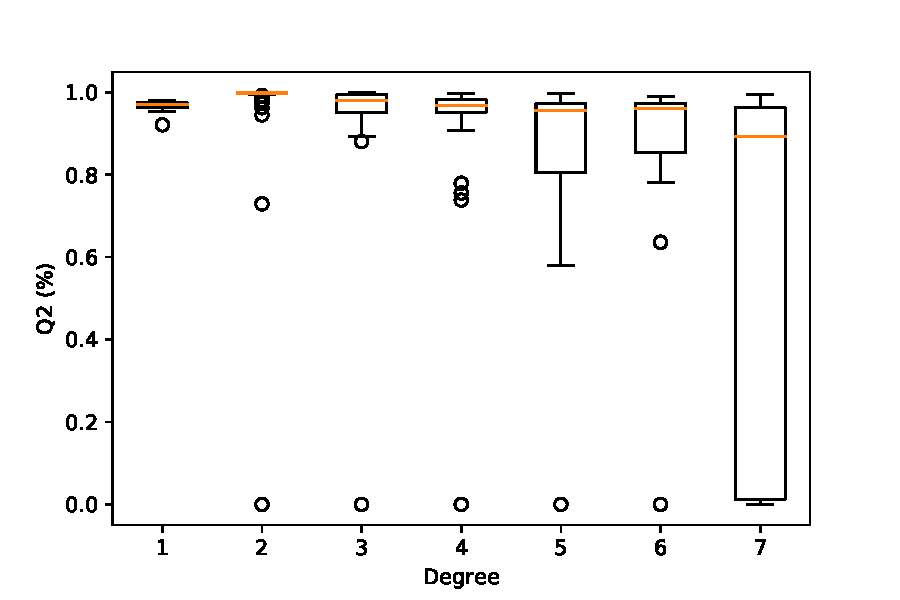
\includegraphics[width=0.45\textwidth]{chaos-poutre-N30-various-degrees.pdf}
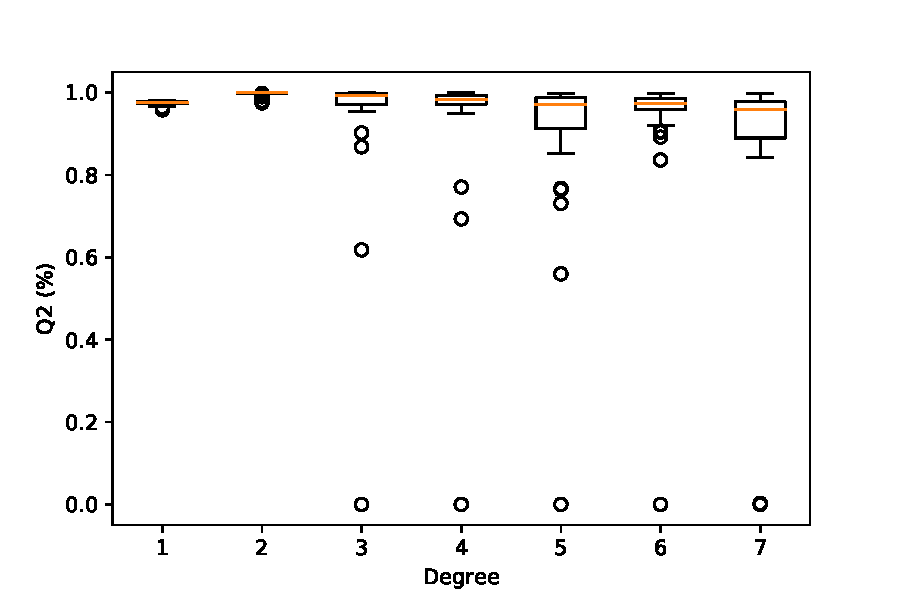
\includegraphics[width=0.45\textwidth]{chaos-poutre-N40-various-degrees.pdf}
\end{center}

Answer:
\begin{itemize}
\item How to set the sample size $n$ ? $n\geq 40$
\item How to set the polynomial degree $d$ ? $d=2$ is the smallest 
degree with high $Q_2$
\end{itemize}


\end{frame}
%%%%%%%%%%%%%%%%%%%%%%%%%%%%%%%%%%%

\begin{frame}[t]{Polynomial chaos example}

\begin{example}
\begin{itemize}
\item Consider the Ishigami model \cite{ishigami1990importance}: 
$$
Y  = \sin(X_1) + a \sin(X_2)^2 + b X_3^4 \sin(X_1)
$$
where $a=7$ and $b=0.1$, with independent marginals: $X_1,X_2,X_3 \sim \mathcal{U}(-\pi, \pi)$.

\item Training sample size: 200, test sample size: 200.
\item We approximate it with \emph{sparse} polynomial chaos: this limits 
the number of coefficients in the model.
\end{itemize}
\end{example}
\end{frame}
%%%%%%%%%%%%%%%%%%%%%%%%%%%%%%%%%%%

\begin{frame}[t]{Polynomial chaos example}

\begin{center}
 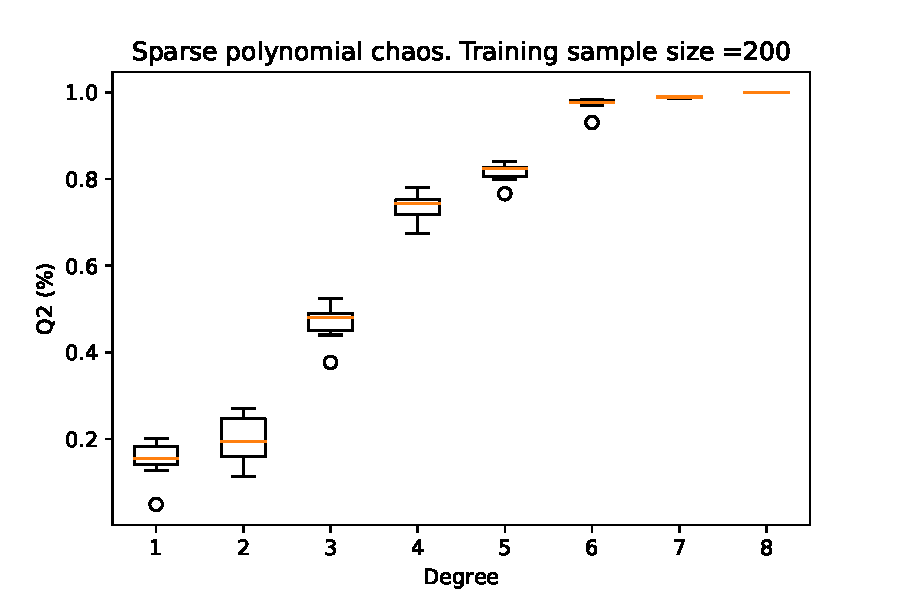
\includegraphics[width=0.8\textwidth]{chaos-ishigami-N200-various-degrees.pdf}
\end{center}

\end{frame}

%%%%%%%%%%%%%%%%%%%%%%%%%%%%%%%%%%%%

\section{References}
\begin{frame}[allowframebreaks]
\frametitle{Références}
\nocite{*}
\bibliographystyle{amsalpha}
\bibliography{Biblio}
\end{frame}

%%%%%%%%%%%%%%%%%%%%%%%%%%%%%%%%%%%%

\section{Appendix}
\begin{frame}
\begin{center}
Appendix
\end{center}
\end{frame}

%%%%%%%%%%%%%%%%%%%%%%%%%%%%%%%%%%%%

\begin{frame}[t]{Some types of metamodels}

{\bf Radial basis function:}
\begin{center}
$\displaystyle{ \tilde{\boldsymbol{Y}} }\,  = \, 
\sum_{k = 1}^{N}  \; \theta_{k} \psi( \left\lVert \boldsymbol{X} - \boldsymbol{X}_k \right\rVert)   $
\end{center}
where $\psi()$ being a radial basis function with its centers taken at $\boldsymbol{X}_k$, $k = 1, \dots N$ in the experimental design

\end{frame}

%%%%%%%%%%%%%%%%%%%%%%%%%%%%%%%%%%%%

\begin{frame}[t]{Some types of metamodels}

{\bf Artificial neural network:}
Radial basis function is a single layer neural network with radial coordinate neurons
\begin{center}
 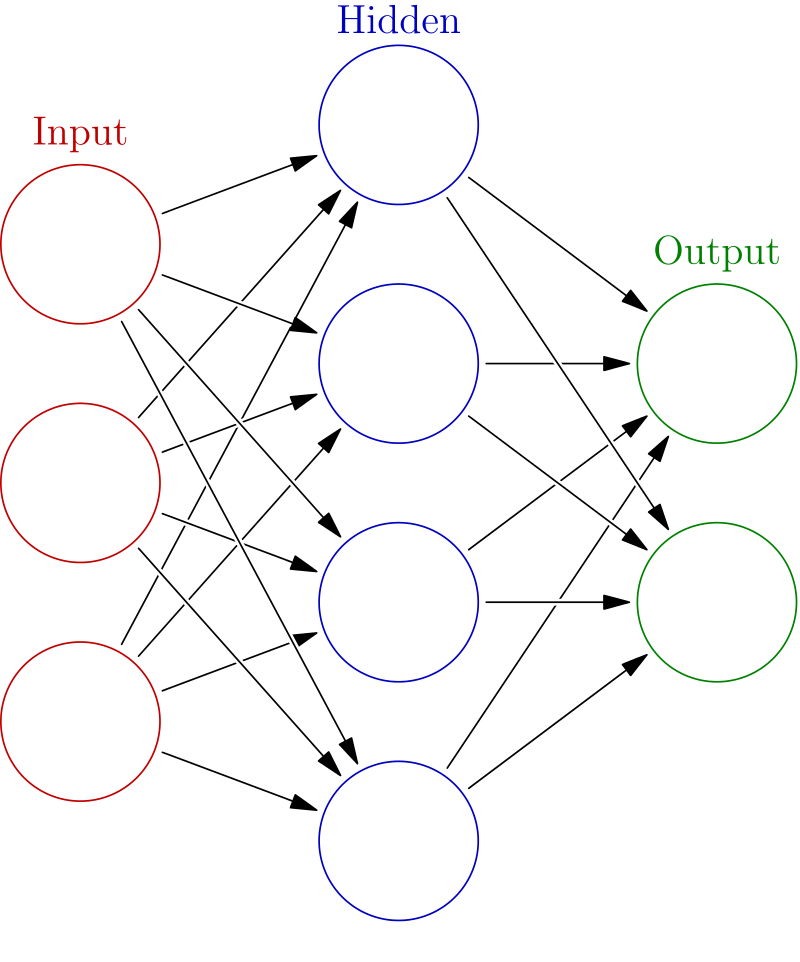
\includegraphics[width=5.0cm]{neural_network.png}
\end{center}

\end{frame}

%%%%%%%%%%%%%%%%%%%%%%%%%%%%%%%%%%%%

\begin{frame}

{\bf Regularized regression methods:} minimize sum of squared errors under a constraint

\[
\boldsymbol{\theta}^* = \arg \min_{\boldsymbol{\theta}} \, \sum_{i=1}^N (Y_i - \hat{f}(\boldsymbol{X}_i, \boldsymbol{\theta}))^2 + \lambda \, R(\boldsymbol{\theta})
\]

\begin{itemize}
\item $R(\boldsymbol{\theta}) = ||\boldsymbol{\theta}||_2$: Ridge regression,
\item $R(\boldsymbol{\theta}) = ||\boldsymbol{\theta}||_1$: LASSO regression,
\item $\lambda$: non-negative regularization coefficient
\end{itemize}

\end{frame}
  
%%%%%%%%%%%%%%%%%%%%%%%%%%%%%%%%%%%%

\section{Methods for fitting metamodels}
\begin{frame}[t]{Methods for fitting metamodels}

{\bf Least square regression:} minimize sum of squared errors of a linear regression model

\[
\boldsymbol{\theta}^* = \arg \min_{\boldsymbol{\theta}} \, \sum_{i=1}^N \epsilon_i^2 =\arg \min_{\boldsymbol{\theta}} \, \sum_{i=1}^N (Y_i - \hat{f}(\boldsymbol{X}_i, \boldsymbol{\theta}))^2
\]

\end{frame}

%%%%%%%%%%%%%%%%%%%%%%%%%%%%%%%%%%%%

\begin{frame}[t]{Methods for fitting metamodels}

{\bf Maximum likelihood estimation:} e.g. assume that the errors $\epsilon$ are independently randomly distributed according to a normal distribution with standard deviation $\sigma$

\[
\mathcal{L}(\btheta) = \frac{1}{ (2 \pi \sigma^2)^{N/2}} \prod_{i=1}^N \exp\left( - \frac{1}{2} \left( \frac{Y_i - \hat{f}(\boldsymbol{X}_i, \boldsymbol{\theta}) }{\sigma} \right) ^2 \right)
\]

\[
\boldsymbol{\theta}^* = \arg \max_{\boldsymbol{\theta}} \, \mathcal{L}(\btheta)
\]
  
\end{frame}

%%%%%%%%%%%%%%%%%%%%%%%%%%%%%%%%%%%%

\begin{frame}[t]{Methods for fitting metamodels}

{\bf $K$-fold cross-validation method:}

$\mathcal{K}: \{1, \dots , N\} \mapsto \{1, \dots, K\}$ partition of $N$ observations to $K$ roughly equal-sized parts, $K=N$: leave-one-out

$\hat{f}^{-k}()$: fitted metamodel with $k$-th part of data set aside

Cross-validation estimate of prediction error:
\begin{center}
$CV(\hat{f}, \boldsymbol{\theta}) = \frac{1}{N} \sum_{i=1}^N L ( Y^i, \hat{f}^{-\mathcal{K}(i)}(X_i) )$
\end{center}

\begin{center}
$
\boldsymbol{\theta}^* = \arg \min_{\boldsymbol{\theta}} \, CV(\hat{f}, \boldsymbol{\theta})
$
\end{center}

\end{frame}

%%%%%%%%%%%%%%%%%%%%%%%%%%%%%%%%%%%%

\section{Some types of metamodels}
\begin{frame}[t]{Some types of metamodels}

{\bf Polynomial models:} (response surface)

Second-order model
\[
\tilde{Y} = \theta_0 + \sum_{i=0}^M \, \theta_i \, X_i + \sum_{i=0}^M \, \theta_{ii} \,X_i^2 + \sum_{i<j} \sum_{j=2}^M \theta_{ij} \,X_i \, X_j
\]

{\bf Polynomial chaos expansion:} 
\begin{center}
$\displaystyle{ \tilde{\boldsymbol{Y}} }\,  = \, 
\sum_{0 \leq |\boldsymbol{k}| \leq p}  \; \theta_{\boldsymbol{k}} \psi_{\boldsymbol{k}}(\boldsymbol{X})  \, $
\end{center}
where $\psi_{\boldsymbol{k}}()$ being polynomial chaos functions

\end{frame}

%%%%%%%%%%%%%%%%%%%%%%%%%%%%%%%%%%%%

\begin{frame}[t]{Some types of metamodels}

{\bf Kriging:} (Gaussian process regression)

Deterministic trend: linear regression on a fixed basis
\[
m(\boldsymbol{X}) = \boldsymbol{r(\boldsymbol{X})}^T \boldsymbol{\theta} 
\]

Random fluctuation: zero-mean stationary Gaussian process of covariance function 
\[
k(\boldsymbol{X}, \boldsymbol{X'}) = \sigma^2 \, \rho( \left\lVert \boldsymbol{X} - \boldsymbol{X'}  \right\rVert)
\]

\end{frame}

\end{document}
